\scanpage{82}

% heading, lines 1–2
Carrés et hexagones dans un pavé

$X$ pavé.

% upper, I), lines 3–6
I) L'ens des carrés $C\subset X$ est en corr $1-1$ avec l'ens (des sommets de) $X$, à tout carré $C$ correspondant l'unique $x\in X$ non lié \deleted{aux sommets} \inserted{à tous les sommets} de $C$, \inserted{et à $a\in C$ l'ens des pts de $C$ non liés à \unsure{$a$}} (\uline{NB} il y a un seul pt de $X$ \inserted{non} lié à \deleted{deux pt} deux pts distincts

% left of upper paragraph
\figure{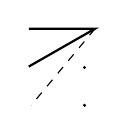
\begin{tikzpicture}[scale=.6]
\draw[thick] (0,1.1)--(1.4,1.1)--(0,.3);\draw[dashed] (1.4,1.1)--(.05,-.52);\fill (1.18,.28) circle (1pt) (1.18,-.52) circle (1pt);
\end{tikzpicture}}

% upper-middle, lines 7–11
non liés -- i.e. \unsure{tte|à} \deleted{\unsure{couple|angle}} \inserted{paire} de pts \deleted{distincts} non liés est contenue dans un trièdre unique -- la donnée d'un tel couple équivaut \inserted{donc} à la donnée d'un trièdre pointée $(t,a)$, en associant à $(t,a)$ la paire $t\setminus\{a\}$ ]

% middle, lines 11–17
Pour que $2$ paires de pts non liés $\{x,x'\}$ $\{y,y'\}$ forment un carré, il faut s. que \deleted{les trièdres} leur ``centre'' $a$ soit le \unsure{$\overline{=}$|$\overline{\mathrm m}$}, i.e qu'elles sont disjointes et \deleted{appartiennent} à deux trièdres \uline{sécants} ; la donnée d'une \deleted{diagonale} des paires $\{x,x'\}$ détermine alors l'autre sans ambiguité ; $\{y,y'\}$ est aussi l'ens des pts de $X$ liés à ceux de $\{x,x'\}$.

% middle left, next to pairs
\diagram{\begin{tikzcd}[ampersand replacement=\&,column sep=tiny,row sep=tiny]
y\arrow[rr,dash]\arrow[dd,dash]\&\&x'\arrow[dd,dash]\\
\&\cdot\&\\
x\arrow[rr,dash]\&\&y'
\end{tikzcd}}

% middle right margin
\figure{\begin{tikzpicture}[x=.16cm,y=.13cm]
\foreach \x/\y in {0/0,1/0,2/0,0/1,1/1,2/1,0/2,1/2,2/2}{\fill[black!55] (\x,\y) circle (.5pt);}
\end{tikzpicture}}

% lower, lines 18–22
Donc la donnée d'un carré à diagonale marquée équivaut à celle d'une paire de pts non liés, ou encore à celle d'une trièdre pointée.

La donnée d'un carré à sommet marqué équivaut à celle d'une trièdre épinglée !

% lower left, three clusters
\figure{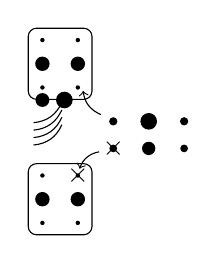
\begin{tikzpicture}[x=.45cm,y=.43cm]
\foreach \off in {0,4}{\draw[rounded corners=3pt] (-.4,\off-.35) rectangle (1.4,\off+1.75);
\foreach \x in {0,1}{\foreach \y in {0,.7,1.4}{\fill (\x,\off+\y) circle (.8pt);}\fill (\x,\off+.7) circle (2.6pt);}}
\node at (1,1.4) {$\times$};
\foreach \x in {2,3,4}{\fill (\x,3) circle (1.5pt);\fill (\x,2.2) circle (1.4pt);}\fill (3,3) circle (3pt) (3,2.2) circle (2.4pt);\node at (2,2.2) {$\times$};\fill (0,3.63) circle (2.5pt) (.62,3.63) circle (3pt);
\draw[->] (1.65,3.2) to[bend left] (1.15,3.9);\draw[->] (1.6,2.1) to[bend right] (1.05,1.6);
\foreach \j in {0,.22,.44,.66}{\draw[thin] (-.25,2.3+\j) to[bend right] (.55,2.9+\j);}
\end{tikzpicture}}

% lower, lines 23–24
\[
\begin{aligned}
\deleted{\unsure{\mathrm{Car}_d}}\quad\mathrm{Car}_d(X)&\simeq\mathrm{triapt}(X)\\
\mathrm{Car}_s(X)&\simeq\mathrm{tria\,ép}(X)\quad\text{(est un $\mathfrak S_3$-ens libre!)}
\end{aligned}
\]

% foot, lines 25–26
\deleted{\unsure{tres|Les autres}} \inserted{Chacun des $4$} pts de $X\setminus C$ distinct du centre $a$ de $C$ est donc lié à exactement un point de la diag $\{x,x'\}$, et

% archive sheet number: 81
